\documentclass[sigconf]{acmart}

\usepackage{graphicx}
\usepackage{hyperref}
\usepackage{todonotes}

\usepackage{endfloat}
\renewcommand{\efloatseparator}{\mbox{}} % no new page between figures

\usepackage{booktabs} % For formal tables

\settopmatter{printacmref=false} % Removes citation information below abstract
\renewcommand\footnotetextcopyrightpermission[1]{} % removes footnote with conference information in first column
\pagestyle{plain} % removes running headers

\newcommand{\TODO}[1]{\todo[inline]{#1}}

\begin{document}
\title{Big Data Applications in the Hospitality Sector}


\author{Neha Rawat}
\affiliation{%
  \institution{Indiana University}
  \city{Bloomington} 
  \state{Indiana} 
}
\email{nrawat@iu.edu}



% The default list of authors is too long for headers}
\renewcommand{\shortauthors}{N. Rawat}


\begin{abstract}
 The rise of {\em Big Data} in the field of Hospitality though recent, is by no means temporary. The hotel industry is one which deals with millions of customers on a day-to-day basis and generates a plethora of customer data through such interactions. It is also the sector which depends the most on customer loyalty, and thus profits greatly through the analytical insights that Big Data has to offer. Keeping this is mind, hotels today, whether they are big chains or small independent establishments, are using data generated internally and on the web to develop strategies for better customer satisfaction, marketing effectiveness, yield management and operational efficiency. 
\end{abstract}

\keywords{i523, HID224, Marketing, Yield Management, Recommendation Systems, Data Warehousing, Data Mining}

\maketitle

\section{Introduction}

Big data is often defined as ``data that exceeds or is beyond the capabilities of the organization to store or analyze for accurate or timely decision making'' \cite {phillipswrenhoskisson01}. It is characterized by features such as its volume, velocity and variety. Two other characteristics that have been recently added to these are veracity and volatility, referring to the uncertainty and dynamic nature of such data \cite {phillipswrenhoskisson01}. Despite the unstructured nature of such data, it presents us with a variety of opportunities which make it so appealing.
\newline The hospitality sector too generates a huge amount of data in its day-to-day processes about its customers, operational processes such as electricity and water consumption and the daily revenue generated. Some of the questions that can be addressed using this data are - What is the country of origin of the customer? What are his/her particular preferences in terms of food or other amenities? What booking channel did they use? What was the time/season of booking? How is the performance of the hotel relative to the local market? What is the monthly energy consumption and other expenditures?\cite {bigdatapredictive02}.
\newline Using the data generated internally by the administrative units and different departments, gathered externally from the web - from sites of aggregators such as Expedia and Trivago and from social networking sites such as Twitter, hotels can derive quite useful insights into the opportunities they can utilize and the challenges they should overcome. 

\section{The advent of Business Intelligence}

Business Intelligence has been a part of the Hospitality sector for some time now. Earlier though, it was used mainly in traditional revenue management systems to deal with duration of stays and promotional programs \cite {kortefrolick03}. However, it was not developed well enough to provide additional insights into other areas of hotel management. The emergence of companies which worked as online booking platforms, such as Expedia and Travelocity, led way to a new form of data, which though unstructured, could be leveraged as a window into the customers' preferences. Few hotels such as Mariott, InterContinental Hotels, Hilton and Hyatt utilized these opportunities presented by business intelligence to get ahead in the game, but were not very successful due to insufficient planning and technical expertise, lack of executive support and wide-spread adoption \cite {kortefrolick03}.

\section{Big Data and Hospitality}

With the advancement of technology, the generation of data increased manifold. Researchers from UC Berkeley had estimated that ``the world had produced about 1.5 billion gigabytes of information in 1999 and in a 2003 replication of the study found out that amount to have doubled in 3 years'' \cite {gpress04}.
\newline The Hospitality sector too found data from a variety of sources - social media, review data, data from search engines like Google and other customer data sources \cite {bigdatapredictive02}. As a result, business intelligence systems were made more structured, driven by advanced IT technologies and machine learning algorithms. Figure 1 gives the structure of a typical hospitality business intelligence system.

\begin{figure}
	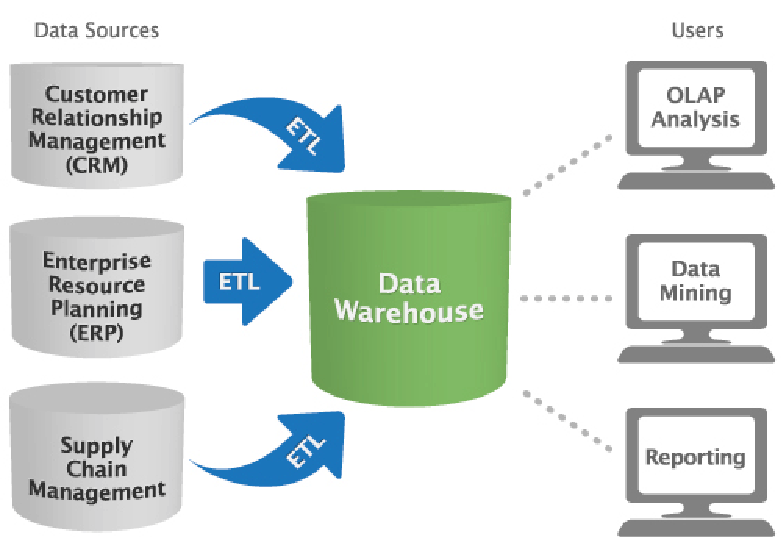
\includegraphics[width=\columnwidth]{images/business_intelligence_system.pdf}
	\caption{Hospitality Business Intelligence System \cite {businessintelligencetools08}}
\end{figure}

The vast amount of data now is used for a variety of tasks in the hotel management field. The most essential ones are - Customer Satisfaction and Marketing, Yield/Revenue Management and Operational Effectiveness.

\subsection{Customer Satisfaction and Marketing}
Customer loyalty is the main driver behind the hospitality business. The use of big data analytics has worked towards providing hoteliers with insights about what their guests want. This information can be used by the hotels to improve existing customer satisfaction as well as develop marketing techniques to attract new customers. This helps convert ``high-spending customers to repeat customers'' and increases the hotel's profitability \cite {mauricio05}.
\newline An excellent example of the use of analytics for customer satisfaction is the new system introduced by the US chain of hotels, Denihan Hospitality \cite {bmarr06}. Using IBM analytics technology, they worked towards combining their internal customer and transactional data with the review data found on the web. This was used to implement various data-driven solutions regarding the quality of the rooms, bathrooms and other facilities. They even went ahead to create interactive dashboards and ``putting analytics in the hands of the frontline hotel staff'' who received real-time updates as to the requirements of their customers \cite {bmarr06}. 
\newline In order to implement the above hotel evaluation structure, one can use the services of WebCrawlers and cloud computing platforms like Hadoop. A similar system created by Ming-Shen Jian, Yi-Chi Fang, Yu-Kai Wang and Chih Cheng uses cloud technologies coupled with data mining algorithms to create a  customer response and evaluation system \cite {jianfangwang07}. The system uses Hadoop to implement a multi-node cluster on the cloud server, programs a  WebCrawler to retrieve review data from websites, extracts the informative adjectives using MapReduce and a text segmentation system and gives the word count using Hadoop's WordCount program. Weights are assigned to the different words using a neural network which are then clustered and analyzed for classification using a clustering algorithm. The final results are averaged for all reviews for a particular hotel to determine its score \cite {jianfangwang07}. Figure 2 gives a rough structure for the above system.

\begin{figure}
	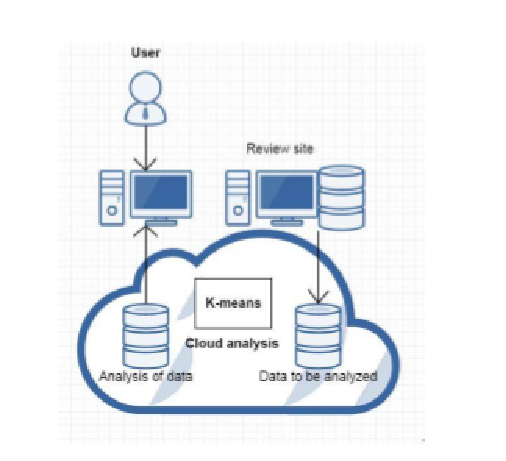
\includegraphics[width=\columnwidth]{images/evaluation_system.pdf}
	\caption{Structure of the Customer Response Evaluation System \cite {jianfangwang07}}
\end{figure}

Marketing too profits from the availability of such data by using search data generated by aggregators such as Expedia and TripAdvisor to develop discount programs and other offers to attract customers. The data history of customers available with hotels can also be used to analyze the requirements of customers at particular times and seasons of the year to create effective marketing strategies. Loyalty programs can be developed to retain long-term customers which can be identified using this data. Events and important occasions can be kept track of in order to release special offers, promotions and advertisements. Data gathered from social media sites is one which can be used most efficiently, through sentiment analysis techniques, to modify marketing strategies according to the different customer demographics.

\subsection{Yield Management}
Yield or Revenue Management deals with price optimization of the different resources offered by a hotel according to different internal as well as external factors. These factors could be the weather or season, the demand and supply in the local market or any internal pricing strategy being implemented.
\newline As mentioned earlier, revenue management was among the first areas where business intelligence was used. Traditional revenue management tools were improved considerably with the advent of big data. Data available on booking sites and on search engines provided different customer channels, resulting in more sources of revenue but also more complexity in the economic management of a hotel. This data however could be leveraged to gain insights about the different customer channels and types so as to align the revenue system accordingly. One example of the above is the {\em innRoad} Real-Time Revenue Management System \cite {bigdatarevenue09}.The innRoad system consists of three components - a forecasting module, a network optimizer and a suite of channel-level optimization modules. It uses real-time data to forecast property demand rates according to different segments and dates and then uses these forecasts for economic evaluation and allocation of rooms. The channel optimization modules use these evaluations along with the data they receive from various channels (rankings, reviews, etc.) to generate real-time prices for different channels, thus providing valuable information regarding the demand and supply view for the hotel \cite {bigdatarevenue09}. Figure 3 gives the architecture for the above revenue management system.

\begin{figure}
	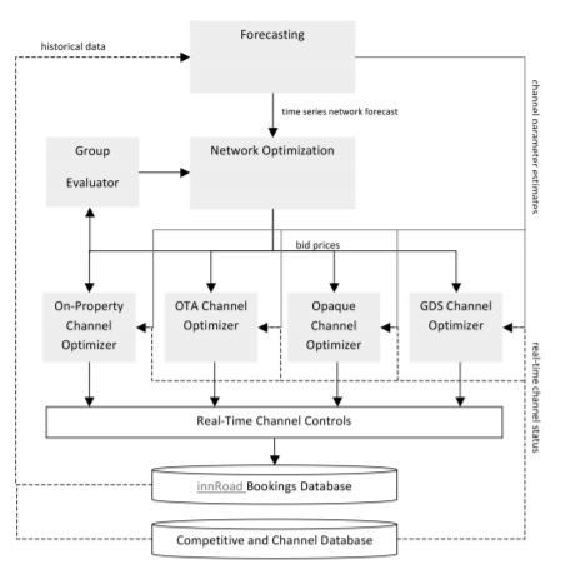
\includegraphics[width=\columnwidth]{images/innRoad.pdf}
	\caption{innRoad Real-Time Revenue Management System \cite {bigdatarevenue09}}
\end{figure}

The result of such an optimized system is an increase in revenue and decrease in management time and effort. The variety of data being generated online can be gathered and structured to create a big data warehouse which can be leveraged by such revenue systems to provide fast and useful real-time business analytic solutions.

\subsection{Operational Effectiveness}
There are several internal operations such as energy and water consumption, which can be optimized to ensure effective resource planning in any hospitality industry. Big data can prove to be a major tool in this area too, especially for big chains. Internal data from hotels belonging to a particular chain can be consolidated and analyzed to gain information about the resource utilization by different hotels and in different areas. Necessary strategies can then be devised to ensure optimum use of resources.
\newline As mentioned by Kahn and Liu, the administrative data from a hotel can act as ``laboratory'' for researching different methods to improve energy efficiency \cite {kahnliu10}. In their study on a major United States hotel chain, they utilized energy consumption data from all hotels in the chain and used a multivariate linear regression technique to understand the factors that affected consumption rate in different areas. One conclusion that they arrived at was that consumption rates were lower in California, which was explained by the stringent energy efficiency laws in California. Conduction of various randomized control-trials also revealed that strategies such as informing people about the downside of increased energy consumption and offering performance bonuses to hotel managers who reduced consumption along with maintaining customer satisfaction, worked in favor of reducing energy costs \cite {kahnliu10}.
\newline The above case study demonstrates how use of even the regular internal energy consumption data generated by hotels over time can prove an essential source of information about the resource utilization in a hotel. Such data mining strategies to contain energy consumption can help decrease not only the operational costs of the hotel but also improve the eco-friendly aspect of the hotel due to reduction of harmful carbon emissions.

\section{Recommendation Systems}
Recommendation systems for travel and hotel sites such as Trivago, Priceline and Expedia are major business intelligence entities in the hospitality sector. These systems deal with huge volumes of data and analyze them to return useful recommendations. The most commonly used recommendation models are - Content-based, Collaborative Filtering and Hybrid. Content-based models provide recommendations based on previous ratings by the user, Collaborative Filtering models provide recommendations based on preferences of similar users and Hybrid models combine the above two i.e. the user's choice as well as the popularity of the recommended hotels \cite {kasr11}.
\newline An example of an effective Collaborative Filtering recommendation system is the KASR (Keyword-Aware Service Recommendation) system \cite {kasr11}. The model was implemented by extracting keywords from user comments to generate a list of keywords which were matched with a domain thesaurus (both for the current user and previous users). Similarity between the current user and any previous user recommendations were calculated using approximate and exact similarity methods. Weights were assigned according to the number of such keywords and personalized ratings were calculated to generate recommendations for the current user. The system was implemented on Hadoop and using MapReduce for better scalability \cite {kasr11}.
\newline Similar to above, recommendation systems for the other two models, using the original algorithm and modified, have also been implemented. These recommendation systems provide users with the convenience of searching and booking optimum travel and stay packages in one go. Hopper, a useful travel application, uses its predictive analytics to inform users of the best time to fly to get cheaper rates on airline tickets. Doing so, it raised 16 million in a growth funding round in 2016 \cite {hopper1613}. Expedia, a well-known travel application, partners with 231,000 hotels and 400 airlines to provide useful deals to customers \cite {expediahopperskyscanner13}. These recommendation systems not only serve as useful tools for their customers but also valuable sources of business data for their client i.e. the hospitality sector.

\section{Case Studies}
Big data analytics has increased tremendously across all service sectors, and the hospitality sector is moving further up the ladder in this era of business intelligence. However, there are a some pioneers which must be mentioned as shining examples in this race. Red Roof Inn, a US economy hotel chain, struck upon the idea of having hotels close to the airport in the winter of 2013-14, as the flight cancellation rates were around 3 per cent at that time and travelers searched for hotels nearby to stay. They used data available publicly regarding flights and weather conditions to launch a marketing strategy that resulted in a 10 per cent increase in business in the targeted areas \cite {bmarr06}. Starwood Hotels and Resorts, a large chain with around 1,200 hotels around the world, used local and worldwide market data along with seasonal weather data to update their pricing system and launch marketing campaigns. This resulted in a 5 per cent increase in their revenue-per-room \cite {bmarr06}. Marriott Hotels, present at over 3,500 locations and generating 12 billion USD in revenue, revealed their success strategy as being ``driven by internet availability''. The launch of the {\em Marriott Reward Program}, based on a business intelligence system which gives real-time information on the member loyalty status, duration of stay, and possible pricing models, has greatly boosted customer satisfaction \cite {kortefrolick03}. InterContinental Hotels in San Fransisco gathered data regarding the energy profiles of their hotel buildings and leveraged it to reduce their energy costs by 10-15 per cent \cite {hotelanalytics14}. Choice Hotels improved their business intelligence program by incorporating {\em Business Objects}, a business intelligence focused company, in their process to attain real-time data about revenue and occupancy rates. The dashboards with all the key data was provided to all their executives to assist in their decisions, thus empowering the company from within using big data analytics as a tool \cite {kortefrolick03}. These case studies truly reflect the impact and growth of big data in the hospitality sector.

\section{Conclusions}
Big Data has revolutionized the field of Travel and Hospitality, and continues to grow as a major factor in all business decisions. What started as a simple revenue management structure, has grown into an intelligent, sustainable system affecting more than one area in the hotel management arena. Launching marketing campaigns, deciding prices and resource allocations, optimizing energy and water consumption, renovating the IT structure, and improving customer comfort and satisfaction, have all been transformed by the arrival of Big Data and business intelligence. There are challenges still to the smooth integration of business intelligence into the day-to-day processes in the Hospitality Industry - overcoming a silos mentality, improving technical expertise to implement the complex Business Intelligence infrastructures needed, and gathering the resources required to support these structures. However, we have observed how the use of big data analytics and intelligence has reformed the hotels who used them. Integration of Big Data and intelligent systems as part of the decision-making process has the potential to become the next `big thing' for the Hospitality Sector.

\bibliographystyle{ACM-Reference-Format}
\bibliography{report} 

\section{Bibtex Issues}
\done[inline]{Warning--no number and no volume in jianfangwang07}
\done[inline]{(There was 1 warning)}
\section{Issues}

\DONE{Example of done item: Once you fix an item, change TODO to DONE}

\subsection{Assignment Submission Issues}

    \TODO{Do not make changes to your paper during grading, when your repository should be frozen.}

\subsection{Uncaught Bibliography Errors}

    \TODO{Missing bibliography file generated by JabRef}
    \TODO{Bibtex labels cannot have any spaces, \_ or \& in it}
    \TODO{Citations in text showing as [?]: this means either your report.bib is not up-to-date or there is a spelling error in the label of the item you want to cite, either in report.bib or in report.tex}

\subsection{Formatting}

    \TODO{Incorrect number of keywords or HID and i523 not included in the keywords}
    \TODO{Other formatting issues}

\subsection{Writing Errors}

    \TODO{Errors in title, e.g. capitalization}
    \TODO{Spelling errors}
    \TODO{Are you using {\em a} and {\em the} properly?}
    \TODO{Do not use phrases such as {\em shown in the Figure below}. Instead, use {\em as shown in Figure 3}, when referring to the 3rd figure}
    \TODO{Do not use the word {\em I} instead use {\em we} even if you are the sole author}
    \TODO{Do not use the phrase {\em In this paper/report we show} instead use {\em We show}. It is not important if this is a paper or a report and does not need to be mentioned}
    \TODO{If you want to say {\em and} do not use {\em \&} but use the word {\em and}}
    \TODO{Use a space after . , : }
    \TODO{When using a section command, the section title is not written in all-caps as format does this for you}\begin{verbatim}\section{Introduction} and NOT \section{INTRODUCTION} \end{verbatim}

\subsection{Citation Issues and Plagiarism}

    \TODO{It is your responsibility to make sure no plagiarism occurs. The instructions and resources were given in the class}
    \TODO{Claims made without citations provided}
    \TODO{Need to paraphrase long quotations (whole sentences or longer)}
    \TODO{Need to quote directly cited material}

\subsection{Character Errors}

    \TODO{Erroneous use of quotation marks, i.e. use ``quotes'' , instead of " "}
    \TODO{To emphasize a word, use {\em emphasize} and not ``quote''}
    \TODO{When using the characters \& \# \% \_  put a backslash before them so that they show up correctly}
    \TODO{Pasting and copying from the Web often results in non-ASCII characters to be used in your text, please remove them and replace accordingly. This is the case for quotes, dashes and all the other special characters.}
    \TODO{If you see a figure and not a figure in text you copied from a text that has the fi combined as a single character}

\subsection{Structural Issues}

    \TODO{Acknowledgement section missing}
    \TODO{Incorrect README file}
    \TODO{In case of a class and if you do a multi-author paper, you need to add an appendix describing who did what in the paper}
    \TODO{The paper has less than 2 pages of text, i.e. excluding images, tables and figures}
    \TODO{The paper has more than 6 pages of text, i.e. excluding images, tables and figures}
    \TODO{Do not artificially inflate your paper if you are below the page limit}

\subsection{Details about the Figures and Tables}

    \TODO{Capitalization errors in referring to captions, e.g. Figure 1, Table 2}
    \TODO{Do use {\em label} and {\em ref} to automatically create figure numbers}
    \TODO{Wrong placement of figure caption. They should be on the bottom of the figure}
    \TODO{Wrong placement of table caption. They should be on the top of the table}
    \TODO{Images submitted incorrectly. They should be in native format, e.g. .graffle, .pptx, .png, .jpg}
    \TODO{Do not submit eps images. Instead, convert them to PDF}

    \TODO{The image files must be in a single directory named "images"}
    \TODO{In case there is a powerpoint in the submission, the image must be exported as PDF}
    \TODO{Make the figures large enough so we can read the details. If needed make the figure over two columns}
    \TODO{Do not worry about the figure placement if they are at a different location than you think. Figures are allowed to float. For this class, you should place all figures at the end of the report.}
    \TODO{In case you copied a figure from another paper you need to ask for copyright permission. In case of a class paper, you must include a reference to the original in the caption}
    \TODO{Remove any figure that is not referred to explicitly in the text (As shown in Figure ..)}
    \TODO{Do not use textwidth as a parameter for includegraphics}
    \TODO{Figures should be reasonably sized and often you just need to
  add columnwidth} e.g. \begin{verbatim}/includegraphics[width=\columnwidth]{images/myimage.pdf}\end{verbatim}

re
\end{document}
